

%%%%%%%%%%%%%%%%%%%%%%%%%%%%%%%%%%%%%%%%%%%%%%%

% ModBus

%%%%%%%%%%%%%%%%%%%%%%%%%%%%%%%%%%%%%%%%%%%%%%%

\chapterimage{pano-tv1.png} % Chapter heading image

\chapter{Modbus}

\section{Introduction}
  \begin{wrapfigure}{r}{3cm}
\Youtube{https://youtu.be/Jj9Tmci7gXU}
\end{wrapfigure}
 \Index{Modbus} est apparu en 1979 à une époque où l'internet n'existait pas encore ! Il est toujours très populaire dans l'industrie. A l'origine Modbus était construit sur un bus série \Index{RS-485} qui connectait différents équipements  appelé (cf. figure~\vref{fig-modbus1})~:
 \begin{itemize}
 \item secondaires ou slaves et 
 \item un primaire appelée aussi master qui gère les communications. 
 \end{itemize}
 
 
 
 \begin{figure}[tbp]
\centerline{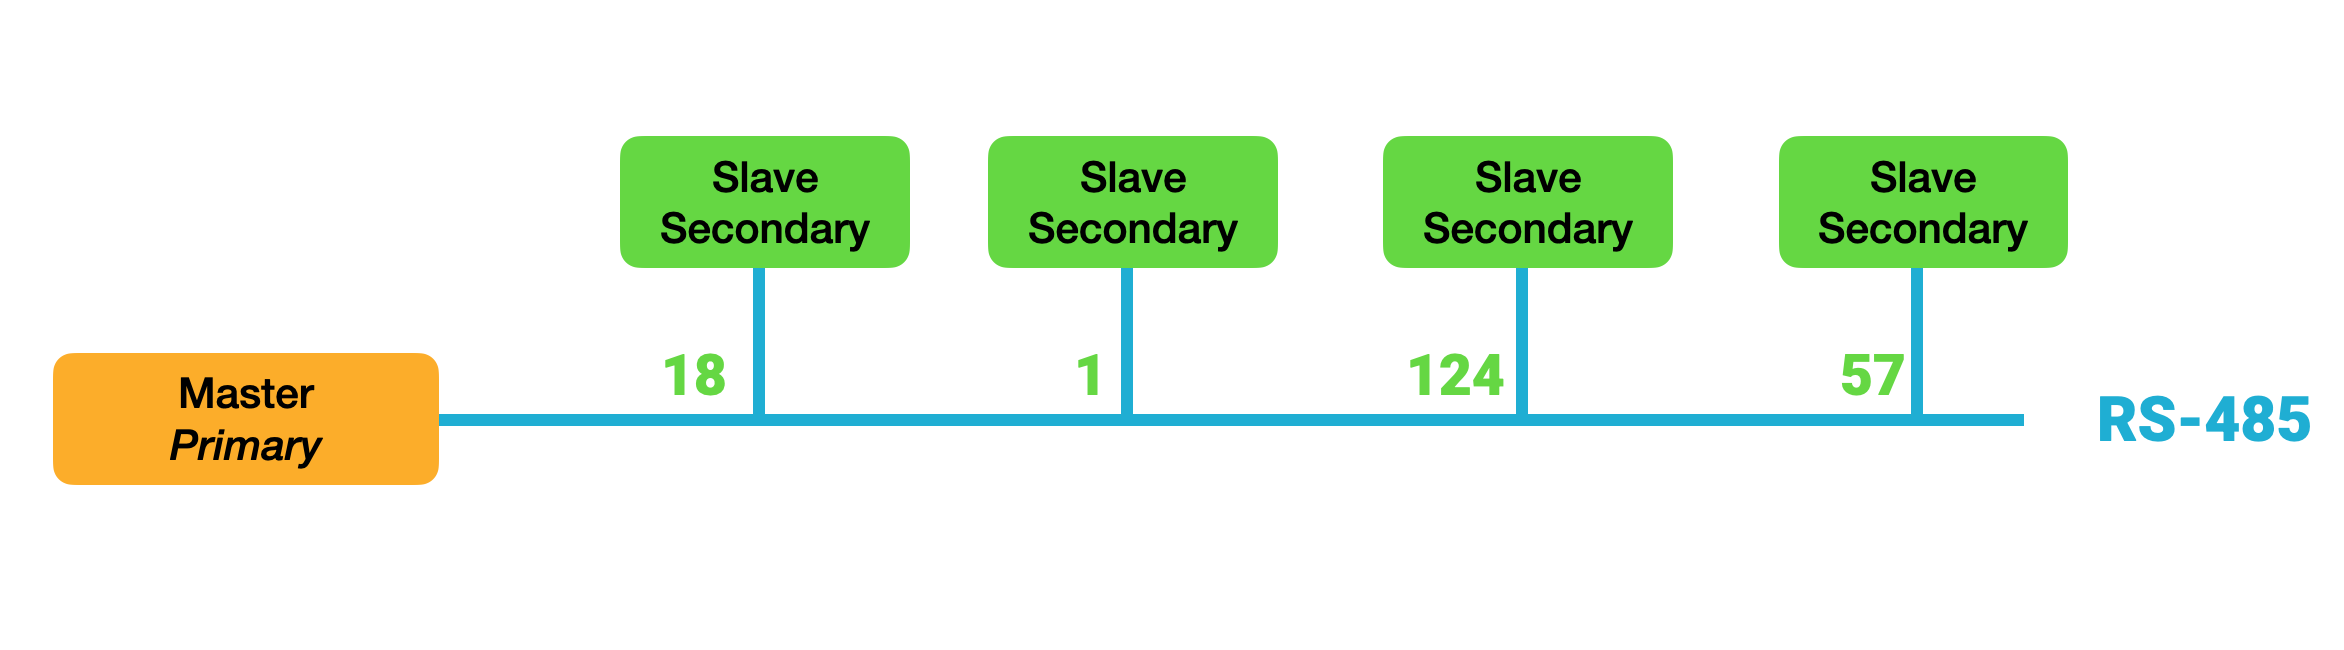
\includegraphics[width=1\columnwidth]{Pictures/Capture35.png}}
\caption{Architecture filaire de Modbus}
\label{fig-modbus1}
\end{figure}

 
 
 Chaque secondaire à un numéro unique ou adresse. Les adresses sont comprises entre 1 et 247. Le primaire n'a pas besoin d'une adresse puisque toutes les communications ont lieu avec lui. 
 
   \vspace{1em}


 Le primaire envoie une requête à un secondaire et le secondaire répond au primaire. Les communications directes entre deux secondaires ne sont pas possibles. 
 
 \subsection{Registres}
 
 
 Un équipement de Modbus peut prendre deux choses à travers des registres : 
 \begin{itemize}
     \item les relais qui peuvent prendre une valeur binaire "on" ou "off". Si le primaire peut modifier l'état et, bien sûr le lire, c'est appeler un \textit{\Index{coil}}. Si la valeur binaire peut uniquement être lu c'est un \textit{\Index{discrete input}}.
     \item des registres sur 16 bits. Ils sont utilisés pour représenter une valeur comme un courant électrique, une température, une vitesse de rotation,... De même, si on peut uniquement lire la valeur à est appelée un \textit{\Index{input register}} sinon, si elle peut être également être modifiée par le primaire, elle est appelée un \textit{\Index{holding register}}.
 \end{itemize}
 
    \vspace{1em}

 
Un équipement Modbus peut avoir jusqu'à 10~000 registres de ces quatre catégories. 

\subsection{Protocole}

Modbus est un protocole requête/réponse. Le primaire envoie une requête à l'adresse d'un équipement pour lire ou écrire un de ces registres. 
\begin{figure}[tbp]
\centerline{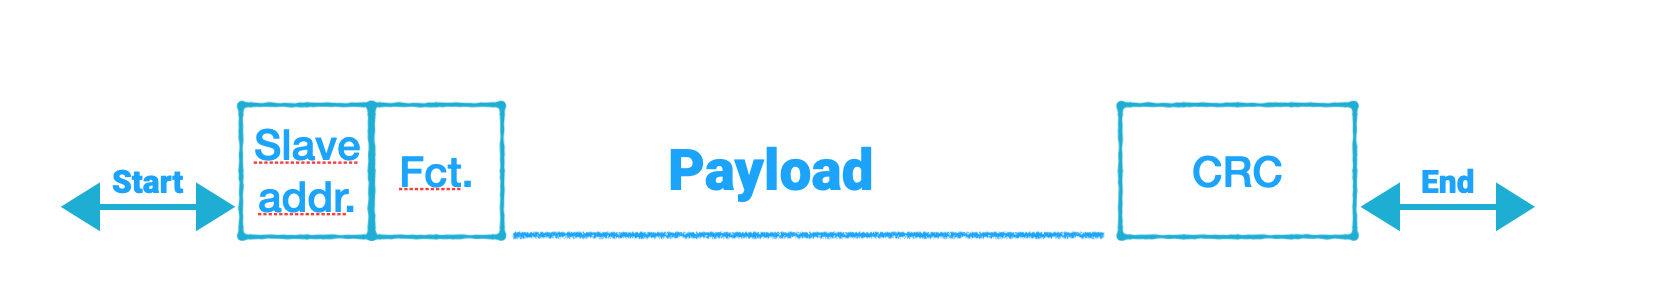
\includegraphics[width=1\columnwidth]{Pictures/Capture37.png}}
\caption{Trame Modbus}
\label{fig-modbus2}
\end{figure}

 

Une trame Modbus est une séquence de caractères commençant par un octet avec l'adresse du secondaire suivi d'une commande ou code de fonctions spécifique à chaque catégorie de registre~:
\begin{itemize}
    \item 1 pour lire un coil,
    \item 2 pour lire un discrete input,
    \item 3 pour lire un holding register,
    \item 4 pour lire un input register,
    \item 5 pour écrire un coil,
    \item 6 pour écrire un holding register,
\end{itemize}

    \vspace{1em}

La suite de la trame contient les données puis un \ac{CRC} pour valider qu'il n'y a pas d'erreur de transmission dans la trame. La partie donnée peut être différente dans la requête et la réponse. Par exemple pour lire un holding register, la requête contient l'adresse du premier registre à lire et le nombre de registres à lire et la réponse contient le nombre de données transmises suivi de leurs valeurs. Pour écrire sur un registre, les données de la trame seront l'adresse du registre et les données à écrire.

\subsection{Exemple: XY-MD02}


Regardons de plus près un exemple concret. On va utiliser un capteur de température et d'humidité, le \Index{XY-MD02} (cf. figure~\vref{fig-XYMD02}) dont les spécifications sont facilement accessibles via une recherche sur Internet. 

\begin{figure}[tbp]
\centerline{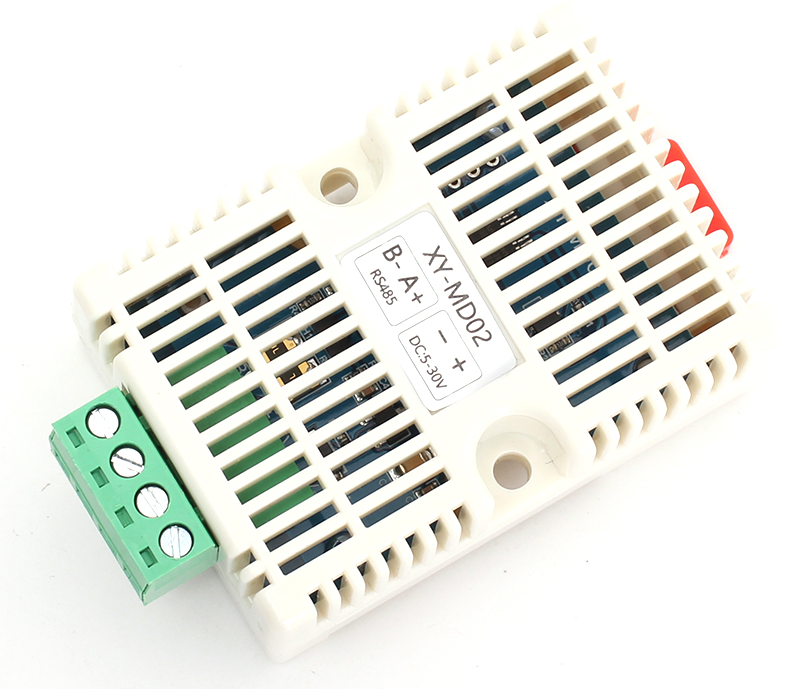
\includegraphics[width=0.5\columnwidth]{Pictures/XY-MD02.png}}
\caption{XY-MD02}
\label{fig-XYMD02}
\end{figure}

La partie verte, se compose de quatre connecteurs dont la signification est indiquée sur l'étiquette. Les deux bornes de gauche constituent le bus \Index{RS-485} nommées \texttt{A+} et \texttt{B-} et les deux bornes de droites permettent d'alimenter électriquement l'équipement avec une tension comprise entre 5V et 30V.

    \vspace{1em}

 \begin{wrapfigure}{r}{3cm}
\Youtube{https://youtu.be/mnRiYaYt2uI}
\end{wrapfigure}

Un adaptateur \Index{USB}/\Index{RS-485} (cf. figure~\vref{fig-USBRS485}) est connecté à un ordinateur. On y retrouve les deux bornes A+ et B- du bus RS-846. L'ordinateur joue le rôle de primaire qui va interroger le capteur de température.  

\begin{figure}[tbp]
\centerline{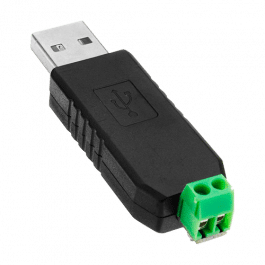
\includegraphics[width=0.3\columnwidth]{Pictures/rs485-usb.png}}
\caption{Adaptateur USB/RS-485}
\label{fig-USBRS485}
\end{figure}

    \vspace{1em}

Le programme \Index{QModMaster}\footnote{\url{https://sourceforge.net/projects/qmodmaster/}} (cf. figure~\vref{fig-qmodmaster}) permet d'interroger ou d'écrire les registres des secondaires. Dans la fenêtre de gauche permet d'accèder aux registres des secondaires. La fenêtre de droite montre le trafic ayant circulé sur le bus RS-485.

\begin{figure}[tbp]
\centerline{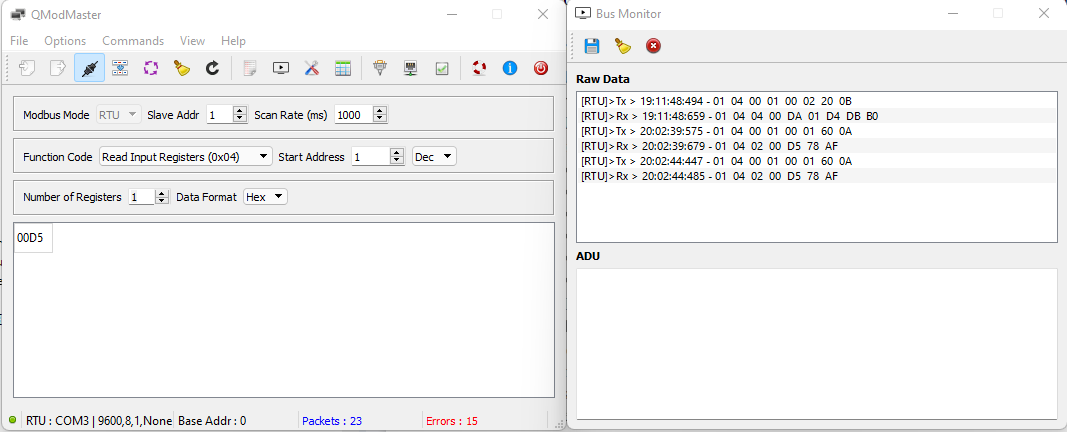
\includegraphics[width=1\columnwidth]{Pictures/modbus-trace.png}}
\caption{QModMaster avec trace des messages}
\label{fig-qmodmaster}
\end{figure}

Pour que le primaire puisse se connecter au secondaire, en plus du nom du port série (ici \texttt{COM3}), il faut disposer de plusieurs informations que l'on peut retrouver dans sa documentation :

\begin{itemize}
    \item la vitesse de transmission sur le bus (ici 9~600 bit/s) et le codage des caractères transmis (ici 8 bits sans bit de parité et un bit de stop)\footnote{\url{https://en.wikipedia.org/wiki/8-N-1}}.
    \item l'adresse du secondaire sur le bus.
\end{itemize}

    \vspace{1em}

La documentation donne également la nature des registres et leur codage. Le tableau~\vref{tab-XY-IR} reprend la définiton des \textit{Input Registers}. Il s'agit de registres qui ne peuvent qu'être lus. La spécification indique que la température est stockée dans le registre 1 sur une longueur de 2 octets, soit l'intégralité de celui-ci.

\begin{table}
\begin{center}
\begin{tabular}{|c|c|c|c|}
\hline
 \rowcolor{purple!10} Register Type & Register Address & Register Contents & Bytes \\ \hline \hline
 \multirow{2}{*}{Input register} & 0x0001 & Temperature & 2 \\ \cline{2-4}
                                 & 0x0002 & Humidity & 2 \\  \hline
\end{tabular}
\end{center}
\caption{Input Register d'un XY-MD02}
\label{tab-XY-IR}
\end{table}

    \vspace{1em}

La documentation indique que le secondaire a l'adresse 0x01 sur le bus RS-485. Il ne reste plus qu'à y envoyer une requête Modbus pour lire ce registre. La fenêtre de trace à droite sur la figure~\vref{fig-qmodmaster} donne les échanges. Nous allons analyser les deux dernières lignes. La première indique le contenu de la requête et la dernière la réponse du secondaire~:

\begin{termc}[backgroundcolor=\color{backcolour}, escapechar=@]
@\texttt{01 \textcolor{blue}{04} \textcolor{purple}{00 01} \textcolor{green!60!black}{00 01} \textcolor{black!30}{60 0A}}@
@\texttt{01 \textcolor{blue}{04} \textcolor{orange}{02} \textbf{00 D5} \textcolor{black!30}{78 AF}}@
\end{termc}

La requête commence par l'adresse du secondaire (\texttt{01}), puis par l'action (\texttt{\textcolor{blue}{04}}) pour lire un \textit{Input Register}, suivit de l'adresse du registre (\texttt{\textcolor{purple}{00 01}}) et du nombre de registres à lire (\textcolor{green!60!black}{00 01}). La requête se termine par la \ac{CRC} validant l'intégrité de la trame (\texttt{\textcolor{black!30}{60 0A}}).

la réponse contient également l'adresse du secondaire (\texttt{01}) et l'action, suivi de la taille de la réponse en octets (\texttt{\textcolor{orange}{02}}) et du résultat demandé (\texttt{\textbf{00 D5}}). 

\Question{Humidité}
{En regardant les échanges de la figure~\vref{fig-qmodmaster} quelle est la valeur mesurée pour l'humidité ?}
{Seul le premier échange demande la lecture de 2 registres à partir du registre ayant l'adresse 0x0001. Dans la réponse on obtient la valeur des deux registres consécutif (\texttt{00 DA} et \texttt{01 D4}). Le tableau~\vref{tab-XY-IR} indique que l'humidité est le second registre, on a donc \texttt{01 D4}.}

Reste à pouvoir interpréter cette valeur. La documentation indique que la valeur est en dixièmes de degrés et que l'unité est le Celsius. En convertissant \texttt{\textbf{00 D5}} en décimal, on obtient 213, soit 21.3\textcelsius.

\Question{Évolution des températures}
{En regardant les échanges de la figure~\vref{fig-qmodmaster} quelle est l'évolution de la température au cours du temps ?}
{On trouve 3 valeurs mesurées à 19:11:48, 20:02:39 et 20:02:44~: \texttt{00 DA}, \texttt{00 D5} et \texttt{00 D5}. Soit 21.8\textcelsius, 21.3\textcelsius ~~et 21.3\textcelsius.}

En résumé, on voit qu'il serait très difficile de faire fonctionner l'équipement sans documentation pour connaître : la vitesse du bus RS-485, l'adresse du secondaire, les adresses des registres utilisés et leur contenu et le codage de l'information dans les registres et les unités utilisées. On a donc un degrés d'interopérabilité faible, les deux entités doivent s'accorder sur un grand nombre de paramètres.

\Question{Taux d'Humidité}
{Quel est le taux d'humidité au moment de la mesure ? La documentation précise qu'il s'agit d'un pourcentage avec une précision au dizième de pourcent. }
{On avait lu la valeur \texttt{01 D4} dans le registre 0x02, soit 468 en décimal. D'où un taux d'humidité de 46.8\%}
    \vspace{1em}

On a pu communiquer avec l'objet en utilisant les paramètres par défaut. Mais pour l'insérer dans un bus, il faut pouvoir modifier certains paramètres. La vitesse de transmission et le codage des octets doit être le même, des secondaires ne peuvent pas avoir la même adresses sur le bus.
Le XY-MD02 dispose aussi de \textit{holding register} permettant de le paramétrage comme le montre la table~\vref{tab-XY-HR}


\begin{table}
\begin{center}
\begin{tabular}{|c|c|c|c|}
\hline
 \rowcolor{purple!10} Register Type & Register Address & Register Contents & Bytes \\ \hline \hline
 \multirow{9}{*}{Holding register} & 0x0101 & Device Address & 2 \\ \cline{2-4}
                                 & 0x1202 & Bit rate: & 2 \\
                                 &        & \tabitem 0~: 9600  & \\
                                 &        & \tabitem 1~: 14400 & \\
                                 &        & \tabitem 2~: 19200 & \\  \cline{2-4}
                                 & 0x0103 & Temperature correction & 2 \\ 
                                 &         & -10\textcelsius ~~- 10\textcelsius &  \\ \cline{2-4}
                                 & 0x0104 & Humidity correction & 2 \\ 
                                 &         & -10\%RH - 10\%RH &  \\ \hline
\end{tabular}
\end{center}
\caption{Holding Register d'un XY-MD02}
\label{tab-XY-HR}
\end{table}

\subsection{Passerelle IP}

\begin{wrapfigure}{r}{8cm}
\centerline{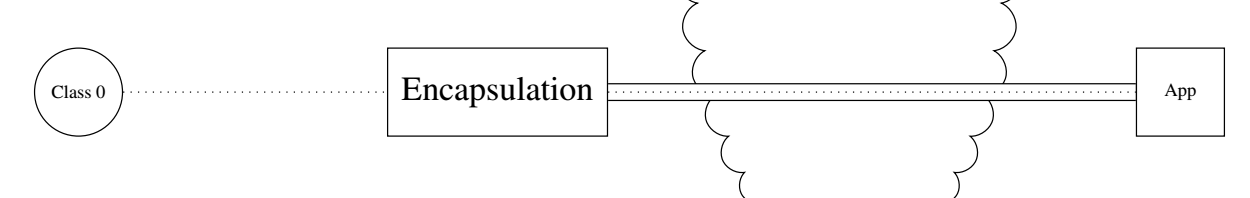
\includegraphics[width=.5\columnwidth]{Pictures/encaps3.png}}
\end{wrapfigure}

Il est possible d'étendre la portée d'un réseau Modbus en ajoutant une passerelle IP. Cela correspond au troisième méthode d'interconnexion de la figure~\vref{fig-encap}. La passerelle, connectée sur le bus où restent connectés les secondaires, possède une adresse IP. Le primaire ouvre une connexion TCP avec la passerelle et y envoie ses requêtes. La passerelle recopie les données sur le bus. Inversement, les réponses des objets sont retournées à la passerelle qui les envoie au primaire en utilisation la connexion TCP. La figure~\vref{fig-gwmodbus} illustre les échanges. On note l'ouverture de connexion TCP qui se fait au démarrage du primaire qui reste active pour toute les échanges. On peut aussi remarquer que les messages TCP sont acquittés. La figure~\vref{fig-msg-modbus} montre les champs commun aux format sur le bus RS-485 et dans des paquets IP.


\begin{figure}
    \centering
    
    \begin{tikzpicture}
    
    %\clip (0.0, 0) rectangle (16,10);
    %\draw[help lines] (0,0) grid (15,9); 
    
    \node[inner sep=0pt] (meter) at (1,7)
        {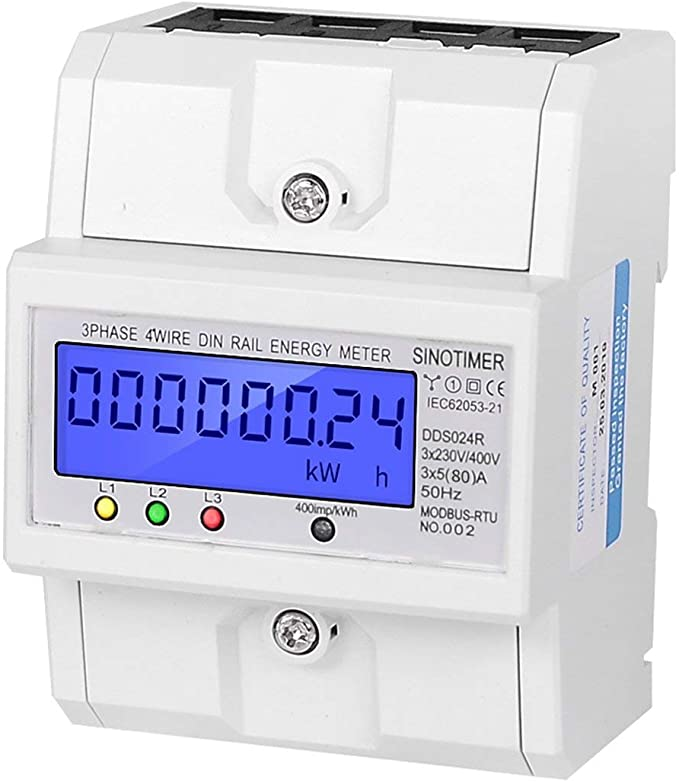
\includegraphics[width=.1\textwidth]{meter.jpg}};
        
    \node[inner sep=0pt] (gw) at (7,7)
        {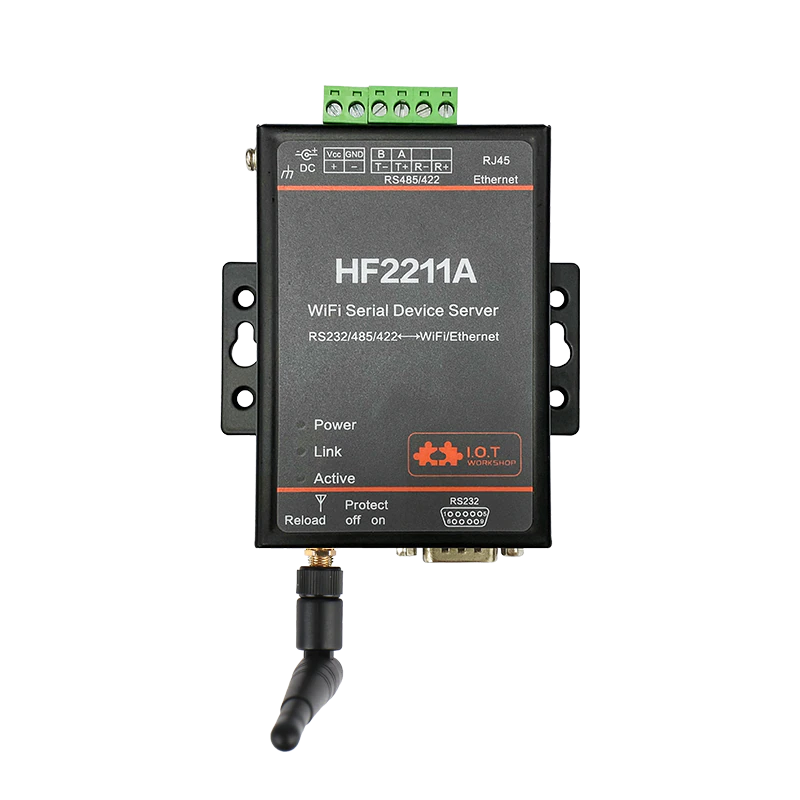
\includegraphics[width=.2\textwidth]{modbusGW2.png}};
    
    \node[inner sep=0pt] (primary) at (13,7)
        {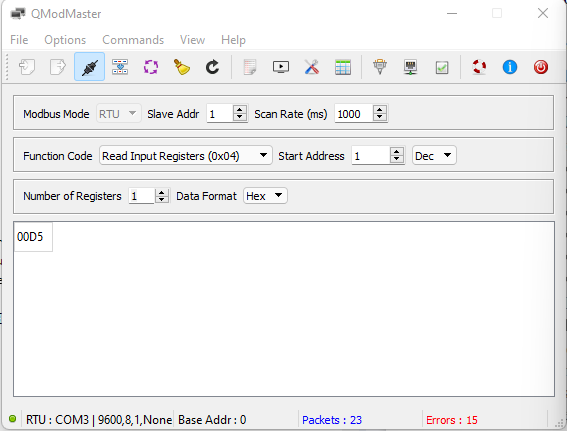
\includegraphics[width=.2\textwidth]{Pictures/QModMaster.png}};
        
        
    \coordinate (tline) at (0, 5.4);
    
    \draw (meter |- tline) node {\small{Compteur}};
    \draw (gw |- tline) node {\small{Passerelle}};
    \draw (primary |- tline) node {\small{Primaire}};
    
    \coordinate (wline) at (0, 8.3);
    
    \draw [decorate, decoration=snake, blue] (meter |- wline) -- coordinate(a)  (gw |- wline);
%    \draw [decorate, decoration={snake}, mirror, yellow] (gw |- wline) -- coordinate(a) (meter);
    
    \draw (a) node [below] {\small{RS-485}};
    
    \path(gw) -- coordinate(b) (primary);
    
    \draw [very thick] ([xshift=0.2cm]gw |- wline) -- coordinate(c) (primary |- wline);
     \draw (c) node [below] {\small{Internet}};
     
     \coordinate(cline) at (0, 5);
     
     \draw [->, thin] (meter |- cline) -- ++ (0, -4) ;
     \draw [->, thin] (gw |- cline) -- ++ (0, -4);
     \draw [->, thin] (primary |- cline) -- ++ (0, -4); 
     
     \draw [thick, ->] ([yshift=-0.1cm] primary |- cline) coordinate (d) -- ([yshift=-0.3cm] gw |- cline) coordinate (e);
     
     \draw (d) node [right] {\tiny{SYN}};
     \draw (e) node [left] {\tiny{SYN/ACK}};
     \draw [thick, ->] (e) -- ([yshift=-0.5cm] primary |- cline) coordinate (f);
     
    \draw (f) node [right] {\tiny{ACK}};
    \draw [thick, ->] (f) -- ([yshift=-0.7cm] gw |- cline) coordinate (h);
    
    \coordinate (tcp_line) at (14.5, 0);
    
    \draw [decoration=brace, decorate] (d -| tcp_line) -- coordinate(i) (h -| tcp_line);
    
    \draw (i) node [below, rotate=90] {\small{Ouverture}};
    
    \draw [double, double distance=0.2cm,] ([yshift=-1.5cm] primary |- cline) coordinate (d) -- ([yshift=-1.7cm] gw |- cline) coordinate (e);
    
    
    \draw  [->] ([yshift=-1.8cm] gw |- cline) -- ([yshift=-2cm] primary |- cline) coordinate(k);
    \draw (k) node [right] {\tiny{ACK}};


    \draw [purple, -> ] ([yshift=-1.5cm] primary |- cline) coordinate (d) -- ([yshift=-1.7cm] gw |- cline);      
    \draw [purple, -> ] ([yshift=-1.7cm] gw |- cline)  -- ([yshift=-2.1cm] meter |- cline) coordinate (e);  

    \draw (d) node [right,purple] {\small{requête}};

    \draw [blue, ] (e) -- ([yshift=-2.5cm] gw |- cline);    
    \draw [double, double distance=0.2cm ] ([yshift=-2.5cm] gw |- cline) -- ([yshift=-2.7cm] primary |- cline);    
    \draw [blue, -> ] ([yshift=-2.5cm] gw |- cline) -- ([yshift=-2.7cm] primary |- cline) coordinate(m);   
    
    \draw  [->] ([yshift=-2.8cm] primary |- cline) -- ([yshift=-3cm] gw |- cline) coordinate(l);
    \draw (l) node [left] {\tiny{ACK}};
    
    \draw (m) node [right,blue] {\small{réponse}};

   
    \end{tikzpicture}
    
    \caption{Passerelle entre le réseau Internet et Modbus.}
    
    \label{fig-gwmodbus}
\end{figure}

\begin{figure}
    \centering
    
    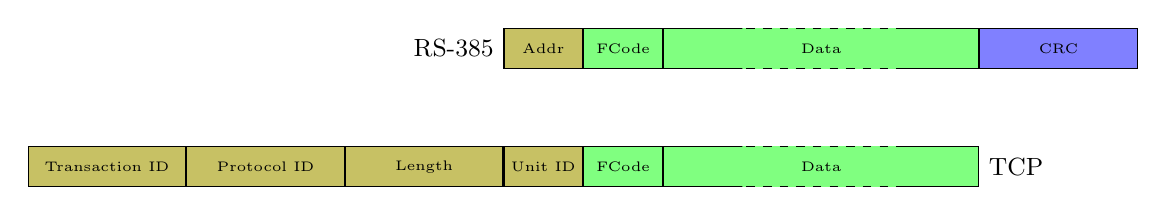
\begin{tikzpicture}
    
  
    
    
    
    \draw (0,0) node (tid) [rectangle, draw,  minimum width = 2cm, minimum height = 0.5cm, fill=olive!50 ] {};
    \draw (tid) node {\tiny{Transaction ID}};


    \draw (tid.east) node (pid) [right, rectangle, draw,  minimum width = 2cm, minimum height = 0.5cm, fill=olive!50 ] {};
    \draw (pid) node {\tiny{Protocol ID}};

    \draw (pid.east) node (len) [right, rectangle, draw,  minimum width = 2cm, minimum height = 0.5cm, fill=olive!50 ] {};
    \draw (len) node {\tiny{Length}};
    
    \draw (len.east) node (uid) [right, rectangle, draw,  minimum width = 1cm, minimum height = 0.5cm, fill=olive!50 ] {};
    \draw (uid) node {\tiny{Unit ID}};

    \draw (uid.east) node (fcode) [right, rectangle, draw,  minimum width = 1cm, minimum height = 0.5cm, fill=green!50 ] {};
    \draw (fcode) node {\tiny{FCode}};
    
    \draw (fcode.east) node (data) [right, rectangle, draw,  minimum width = 4cm, minimum height = 0.5cm, fill=green!50 ] {};
    \draw (data) node {\tiny{Data}};
    
    \draw [green!50] (data.north) -- +(-1, 0) -- +(1, 0);
    \draw [green!50] (data.south) -- +(-1, 0) -- +(1, 0);
    \draw [dashed] (data.north) -- +(-1, 0) -- +(1, 0);
    \draw [dashed] (data.south) -- +(-1, 0) -- +(1, 0);
    
    \draw (data.east) node [right] {\small{TCP}};
    
    
    \path (uid.west) -- ++(0, 1.5) coordinate(x);
    \draw (x) node (addr) [right, rectangle, draw,  minimum width = 1cm, minimum height = 0.5cm, fill=olive!50 ] {};
    \draw (addr) node {\tiny{Addr}};  

   \draw (addr.east) node (fcode) [right, rectangle, draw,  minimum width = 1cm, minimum height = 0.5cm, fill=green!50 ] {};
    \draw (fcode) node {\tiny{FCode}};
    
    \draw (fcode.east) node (data) [right, rectangle, draw,  minimum width = 4cm, minimum height = 0.5cm, fill=green!50 ] {};
    \draw (data) node {\tiny{Data}};    
   \draw [green!50] (data.north) -- +(-1, 0) -- +(1, 0);
    \draw [green!50] (data.south) -- +(-1, 0) -- +(1, 0);
    \draw [dashed] (data.north) -- +(-1, 0) -- +(1, 0);
    \draw [dashed] (data.south) -- +(-1, 0) -- +(1, 0);
    

    \draw (data.east) node (crc) [right, rectangle, draw,  minimum width = 2cm, minimum height = 0.5cm, fill=blue!50 ] {};
    \draw (crc) node {\tiny{CRC}};
    
    \draw(x) node [left] {\small{RS-385}};
    \end{tikzpicture}
    
    \caption{Messages Modbus sur bus RS-485 et sur IP/TCP}
    
    \label{fig-msg-modbus}
\end{figure}


Comme dans l'exemple précédent du capteur de température, les spécifications du \Index{compteur électrique} sont nécessaires pour comprendre la signification des registres utilisables. Le compteur code ses valeurs sur des nombres flottant sur 32 bits dont le codage est spécifié par la norme \Index{IEEE 754}\footnote{\url{https://en.wikipedia.org/wiki/IEEE_754}}. Ces valeurs sur 32 bits doivent être codées sur deux registres consécutifs d'où l'incrémentation de 2 en 2 que l'on retrouve sur la tableau~\vref{tab-meter-IR}, le compteur pouvant mesurer trois phase électriques.


\begin{table}
\begin{center}
\begin{tabular}{|c|c|c|c|c|}
\hline
 \rowcolor{purple!10} Register Type & Register Address & Register Contents & Unité & Format \\ \hline \hline
 \multirow{10}{*}{Input register} & 0x0000 & \Index{Voltage} phase A & V &  IEEE 754 \\ \cline{2-5}
                                 & 0x0002 & Voltage phase B & V &  IEEE 754 \\ \cline{2-5}
                                 & 0x0004 & Voltage phase C & V &  IEEE 754 \\ \cline{2-5}
                                 & 0x0008 & \Index{Intensité} phase A & A &  IEEE 754 \\ \cline{2-5}
                                 & 0x000A & Intensité phase B & A &  IEEE 754 \\ \cline{2-5}
                                 & 0x000C & Intensité phase C & A &  IEEE 754 \\ \cline{2-5}
                                 & 0x0010 & \Index{Puissance} Totale & KWh &  IEEE 754 \\ \cline{2-5}
                                 & 0x0012 & Puissance phase A & KWh &  IEEE 754 \\ \cline{2-5}
                                 & 0x0014 & Puissance phase B & KWh &  IEEE 754 \\ \cline{2-5}
                                 & 0x0016 & Puissance phase C & KWh &  IEEE 754 \\ \cline{2-5}
                                 & 0x0036 & \Index{Fréquence} & Hz &  IEEE 754 \\ \hline

\end{tabular}
\end{center}
\caption{quelques \textit{Input Register} du compteur électrique}
\label{tab-meter-IR}
\end{table}

    \vspace{1em}

\Index{Wireshark} peut capturer une requête ayant circulé sur le réseau Ethernet, coté primaire (cf. figure~\vref{fig-modbus-ws}).

\begin{figure}[tbp]
\centerline{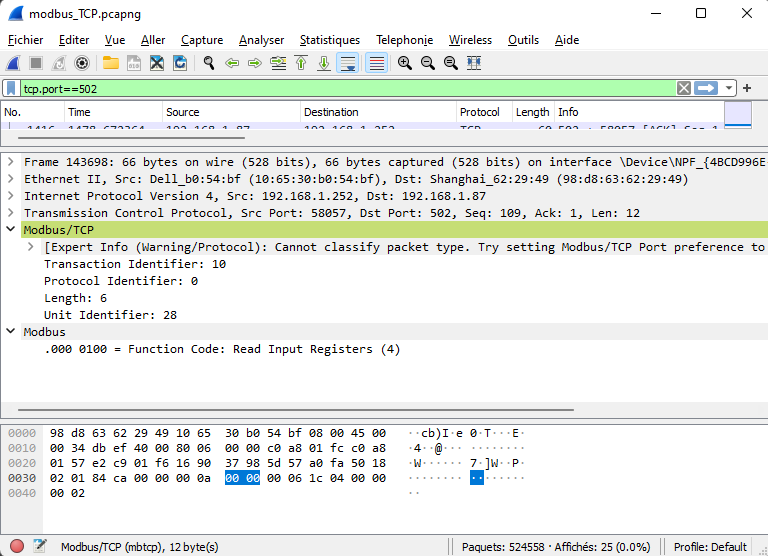
\includegraphics[width=1\columnwidth]{Pictures/modbus-ws.png}}
\caption{Capture avec \Index{Wireshark} d'une trame contenant un message Modbus.}
\label{fig-modbus-ws}
\end{figure}


\begin{termc}[backgroundcolor=\color{backcolour}, escapechar=#]
#\texttt{\small{0000 \colorbox{purple!50}{98 d8 63 62 29 49 10 65 30 b0 54 bf 08 00}\colorbox{blue!30}{45 00}   ..cb)I.e0.T...E.}}#
#\texttt{\small{0010  \colorbox{blue!30}{00 34 db ef 40 00 80 06 00 00 c0 a8 01 fc c0 a8}   .4..@...........}}#
#\texttt{\small{0020  \colorbox{blue!30}{01 57}\colorbox{red!30}{e2 c9 01 f6 16 90 37 98 5d 57 a0 fa 50 18}   .W......7.]W..P.}}#
#\texttt{\small{0030  \colorbox{red!30}{02 01 84 ca 00 00} \ul{00 0a} \ul{00 00} \ul{00 06} 1c \textcolor{blue}{04} \textcolor{red}{00 00}   ................}}#
#\texttt{\small{0040  \textcolor{green}{00 02}   ..              }}#                                 
\end{termc}

On retrouve les encapsulations des protocoles Ethernet, IP et TCP, suivi des données TCP. Elles se composent de  trois champs qui n'existent pas dans la requête circulant sur le bus RS-485~:
\begin{itemize}
    \item le numéro de la transaction sur deux octets incrémenté à chaque requête,
    \item la version du protocole sur deux octets, 
    \item la longueur en octet de la transaction.
\end{itemize}

    \vspace{1em}

Les champs suivants sont identiques à ceux de la trame sur le bus RS-485~:
\begin{itemize}
    \item l'adresse du secondaire sur un octet, ici 0x1c ou 28,
    \item la nature de la requête : 0x04 pour lire un input register,
    \item le registre à lire sur deux octets, ici 0x0000 correspondant à la tension sur la phase A.
    \item le nombre de registre à lire, ici 2 pour obtenir les 32 bits de la valeur.
\end{itemize}

    \vspace{1em}

Le primaire reçoit la réponse suivante~:

\begin{termc}[backgroundcolor=\color{backcolour}, escapechar=#]
#\texttt{\small{0000  \colorbox{purple!50}{10 65 30 b0 54 bf 98 d8 63 62 29 49 08 00}\colorbox{blue!30}{45 00}   .e0.T...cb)I..E.}}# 
#\texttt{\small{0010  \colorbox{blue!30}{00 35 c9 75 00 00 40 06 2c aa c0 a8 01 57 c0 a8}   .5.u..@.,....W..}}# 
#\texttt{\small{0020  \colorbox{blue!30}{01 fc}\colorbox{red!30}{01 f6 e2 c9 5d 57 a0 fa 16 90 37 a4 50 18}   ......]W....7.P.}}# 
#\texttt{\small{0030  \colorbox{red!30}{44 70 e1 6e 00 00} \ul{00 0a} \ul{00 00} \ul{00 07} 1c \textcolor{blue}{04} \textcolor{orange}{04}\colorbox{black}{\textcolor{white}{43}}   Dp.n...........C}}# 
#\texttt{\small{0040  \colorbox{black}{\textcolor{white}{69 9e 4a}} \ \ \ \ \ \ \ \ \ \ \ \ \ \ \ \ \ \ \ \ \ \ \ \ \ \ \ \ \ \ \ \ \ \ \ \ \ \ \ i.J}}# 
                           
\end{termc}

On y retrouve, après les encapsulations protocolaires d'Ethernet, IP et TCP les données suivantes~:
\begin{itemize}
    \item le numéro de transaction qui correspond à celui employé dans la requête précédente. cela permet de faire le lien entre les deux messages qui aurait pu se defaire en cas de perte de paquets sur le réseau Internet,
    \item la version du protocole,
    \item la longueur de la réponse, ici 7 octets,
    \item l'adresse du secondaire ayant répondu, ici 28,
    \item la nature de la requête,
    \item le nombre d'octets retournés, ici 4,
    \item et la valeur des deux registres \texttt{0x43699e4a} qui correspond à un nombre flottant tel que le représente le standard IEEE 754. Il existe de nombreux sites sur Internet qui permettent la conversion\footnote{\url{https://www.h-schmidt.net/FloatConverter/IEEE754.html}}. Comme le montre la figure~\vref{fig-ieee754}, on obtient la valeur \SI{233.61831665}\volt qui correspond bien à une tension offerte par un réseau électrique.
\end{itemize}

  \begin{figure}[tbp]
\centerline{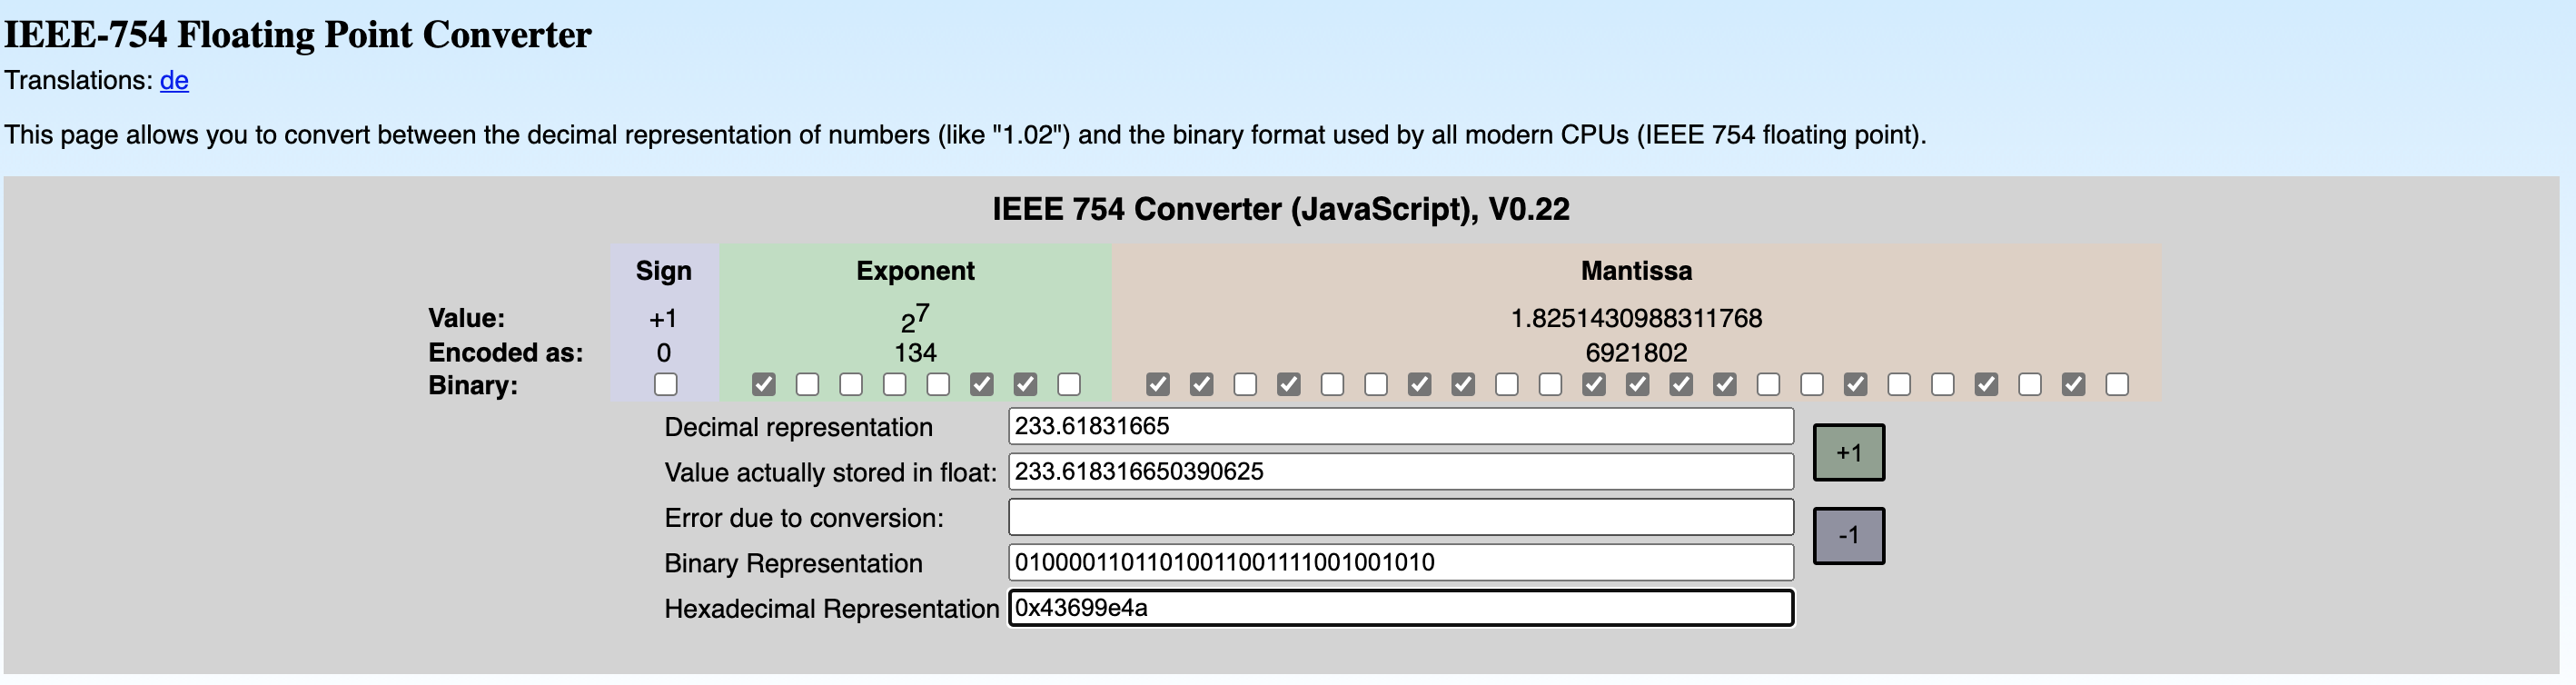
\includegraphics[width=1\columnwidth]{Pictures/IEEE754.png}}
\caption{Conversion d'un nombre flottant}
\label{fig-ieee754}
\end{figure}

\Question{Requête Modbus TCP}
{Soit l'échange donné figure~\vref{fig-exo-ws} correspondant à une requête Modbus et à une réponse.
Quel est le numéro de port utilisé par Modbus TCP.}
{Il y a deux ports dasn l'en-tête TCP, mais comme il s'agit d'une requête, il faut prendre le port destination~:0x1f6, soit 502 en décimal}

\Question{Requête Modbus TCP}
{En poursuivant l'analyse du trafic, quelle valeur de registre est demandée.}
{Le registre 0x36 est demandé, en regardant dans la table~\vref{tab-meter-IR}, il s'agit de la fréquence en Hz}

\Question{Réponse Modbus TCP}
{En analysant le paquet suivant, 
Comment peut-on vérifier que la réponse peut correspondre à la requête précédente.}
{Le numéro de séquence 0x000c est le même dans les deux trames.}


\Question{Réponse Modbus TCP}
{Quelle valeur est retournée. Est-ce cohérent ?}
{La valeur du registre est 0x4247e95b correspond à un nombre flottant IEEE 754, en convertissant on obtient la valeur 49.9778862 Hz qui est très proche de la fréquence du réseau électrique européen.}

\begin{figure}[tbp]

\begin{termc}[backgroundcolor=\color{backcolour}, escapechar=#]
#\texttt{\small{0000  \colorbox{purple!50}{98 d8 63 62 29 49 10 65 30 b0 54 bf 08 00}\colorbox{blue!30}{45 00}   ..cb)I.e0.T...E.}}#
#\texttt{\small{0010  \colorbox{blue!30}{00 34 db f3 40 00 80 06 00 00 c0 a8 01 fc c0 a8}   .4..@...........}}#
#\texttt{\small{0020  \colorbox{blue!30}{01 57}\colorbox{red!30}{e2 c9 01 f6 16 90 37 b0 5d 57 a1 14 50 18}   .W......7.]W..P.}}#
#\texttt{\small{0030  \colorbox{red!30}{02 01 84 ca 00 00} 00 0c 00 00 00 06 1c 04 00 36   ...............6}}#
#\texttt{\small{0040  00 02 \ \ \ \ \ \ \ \ \ \ \ \ \ \ \ \ \ \ \ \ \ \ \ \ \ \ \ \ \ \ \ \ \ \ \ \ \ \ \ \ \ \  ..}}#
                           
\end{termc}

\begin{termc}[backgroundcolor=\color{backcolour}, escapechar=#]
#\texttt{\small{0000  \colorbox{purple!50}{10 65 30 b0 54 bf 98 d8 63 62 29 49 08 00}\colorbox{blue!30}{45 00}   .e0.T...cb)I..E.}}#
#\texttt{\small{0010  \colorbox{blue!30}{00 35 8b 15 00 00 40 06 6b 0a c0 a8 01 57 c0 a8}   .5....@.k....W..}}#
#\texttt{\small{0020  \colorbox{blue!30}{01 fc}\colorbox{red!30}{01 f6 e2 c9 5d 57 a1 14 16 90 37 bc 50 18}   ......]W....7.P.}}#
#\texttt{\small{0030  \colorbox{red!30}{44 70 f1 f0 00 00} 00 0c 00 00 00 07 1c 04 04 42   Dp.............B}}#
#\texttt{\small{0040  47 e9 5b \ \ \ \ \ \ \ \ \ \ \ \ \ \ \ \ \ \ \ \ \ \ \ \ \ \ \ \ \ \ \ \ \ \ \ \ \ \ \ \  G.[}}#
                           
\end{termc}
\caption{Capture à étudier.}
\label{fig-exo-ws}
\end{figure}